\documentclass[onecolumn, draftclsnofoot,10pt, compsoc]{IEEEtran}
\usepackage{graphicx}
\usepackage{url}
\usepackage{setspace}
\usepackage{pgfgantt}
\usepackage{geometry}
\geometry{textheight=9.5in, textwidth=7in}

% 1. Fill in these details
\def \CapstoneTeamName{		Project LOOM}
\def \CapstoneTeamNumber{		36}
\def \GroupMemberOne{			William Selbie}
\def \GroupMemberTwo{			Trevor Swope}
\def \GroupMemberThree{			Luke Goertzen}
\def \CapstoneProjectName{		Project LOOM | Design an Internet of Things Rapid Prototyping System.}
\def \CapstoneSponsorCompany{	}
\def \CapstoneSponsorPerson{		Chet Udell}

% 2. Uncomment the appropriate line below so that the document type works
\def \DocType{	%Problem Statement
				Requirements Document
				%Technology Review
				%Design Documeet
				%Progress Report
				}
			
\newcommand{\NameSigPair}[1]{\par
\makebox[2.75in][r]{#1} \hfil 	\makebox[3.25in]{\makebox[2.25in]{\hrulefill} \hfill		\makebox[.75in]{\hrulefill}}
\par\vspace{-12pt} \textit{\tiny\noindent
\makebox[2.75in]{} \hfil		\makebox[3.25in]{\makebox[2.25in][r]{Signature} \hfill	\makebox[.75in][r]{Date}}}}
% 3. If the document is not to be signed, uncomment the RENEWcommand below
\renewcommand{\NameSigPair}[1]{#1}

%%%%%%%%%%%%%%%%%%%%%%%%%%%%%%%%%%%%%%%
\begin{document}
\begin{titlepage}
    \pagenumbering{gobble}
    \begin{singlespace}
        \hfill 
        % 4. If you have a logo, use this includegraphics command to put it on the coversheet.
        %\includegraphics[height=4cm]{CompanyLogo}   
        \par\vspace{.2in}
        \centering
        \scshape{
            \huge CS Capstone \DocType \par
            {\large\today}\par
            \vspace{.5in}
            \textbf{\Huge\CapstoneProjectName}\par
            \vfill
            {\large Prepared for}\par
            \Huge \CapstoneSponsorCompany\par
            \vspace{5pt}
            {\Large\NameSigPair{\CapstoneSponsorPerson}\par}
            {\large Prepared by }\par
            Group\CapstoneTeamNumber\par
            % 5. comment out the line below this one if you do not wish to name your team
            \CapstoneTeamName\par 
            \vspace{5pt}
            {\Large
                \NameSigPair{\GroupMemberOne}\par
                \NameSigPair{\GroupMemberTwo}\par
                \NameSigPair{\GroupMemberThree}\par
            }
            \vspace{20pt}
        }
%        \begin{abstract}
% 6. Fill in your abstract    
%        	Our project involves creating a rapid prototyping system in the field of Internet of Things that can be used by those with minimal technical experience, with specific focus on use in the field of agriculture.
%			This will take the form of modular hardware kits that can be programmed using a graphical interface so that the user never has to write a line of code. The reason that this is so useful is because of the current barriers to entry for Internet of Things type solutions greatly restrict the quantity of solutions being proposed. At the same time, Internet of Things related ideas have the potential to solve a large quantity of problems, but a lot of the population lacks the technical skills to enact these solutions even though they have the creativity to come up with them. 
%			By giving those without technical experience the ability to create and build their own solutions we are removing one of the barriers to entry to creating Internet of Things type solutions, resulting, in theory, in a greater number of problems being solved. 
%       \end{abstract}     
    \end{singlespace}
\end{titlepage}
\newpage
\pagenumbering{arabic}
\tableofcontents
% 7. uncomment this (if applicable). Consider adding a page break.
%\listoffigures
%\listoftables
\clearpage

% 8. now you write!
\section{Introduction}
	\subsection{Purpose}
	This document aims to elucidate the goals, scope, requirements, and development process of the software and hardware of Project LOOM. Project LOOM will be a modular suite of Internet of Things devices whose extensible and easy programmability expands the demographic of people capable of implementing Internet of Things solutions.
	\subsection{Scope}
	With Project LOOM, we aim to create an open-source, plug-and-play suite of modular building blocks that can be used by a user with limited technical expertise to create complex systems. We hope to broaden the range of people capable of implementing IoT projects by developing a system that abstracts out the more technical details consistent to any project.
	\subsection{Definitions, Acronyms, and Abbreviations}
	\textbf{The Internet of Things (IoT):} Entails an aggregate of embedded systems capable of reading, transmitting, receiving, processing, and acting upon data. This often takes the form of a network of remotely connected devices that can be used for the purpose of autonomous data collection, or remote control and automation of various systems. \newline
	\textbf{Module:} An interchangeable, self-contained device that can be connected to an IoT network with minimal configuration. Connects to other modules to combine behaviors (i.e. a sensor attached to a WiFi adapter becomes a sensor that transfers data over WiFi). \newline
	\textbf{Gateway:} A wired or wireless node connecting multiple devices on a network (e.g. WiFi, Ethernet) \newline
	\textbf{Long-Range Wireless Radio Frequency (LoRa RF or just LoRa):} A flavor of gateway that transmits over 2-26km line of sight

	\subsection{References}
	List that Gantt chart exists (actual chart lives elsewhere)
	\subsection{Overview}
	The remainder of the document will provide more specific information regarding the functions and constraints of Project LOOM, as well as characteristics of its users and the assumptions and dependencies that are inherent to its inception. 

\section{Overall Description}
	\subsection{Product Perspective}
	The part of Project LOOM being worked on by Group 36 is merely a subset of the larger project that includes developing the graphical interface that will be used to program the kits as well as the embedded firmware that will be run on the devices themselves.

	\subsubsection{User Interfaces}
	The main user interface will be a module for MaxMSP that 
	\subsection{Product Functions}
		\begin{itemize}
		\item The product must be able to receive and transmit data with physically and wirelessly connected modules.
		\item Users must be able to view the readings or actions of the connected modules via software
		\item Users must be able to remotely trigger events on actuators
		\item Users must be able to re-calibrate devices remotely
		\item Users must be able to program the devices with the Arduino development environment by altering or replicating the open-source code on which the firmware is based.
		\end{itemize}

	\subsection{User Characteristics}
	There are a range of possible users for the LOOM devices and software; the target audience is meant to span from novice hobbyists to experts. Anyone wanting to learn about or implement an IoT solution in a streamlined fashion should be able to pick it up out of the box and get a simple system working without any programming. On the other end of the spectrum, there are users with more technical expertise, who simply want well-designed sensors and actuators that work together in a way that make sense. Since Project LOOM is open-source, these users will be able to write their own software and firmware for the chips if they choose to do so.
	Project LOOM is currently being developed with the intent to be tested by university professors and their students.

	\subsection{Constraints}
		\begin{enumerate}
			\item \textbf{Regulatory policies:} FCC.
			\item \textbf{Hardware limitations (e.g., signal timing requirements):} AdaFruit FeatherM0, MPU6050
			\item \textbf{Interfaces to other applications:} Connection to MaxMSP via serial/WiFi/other Gateway
			\item \textbf{Parallel operations:} Sending/receiving at the same time
			\item \textbf{Audit functions:} Not relevant
			\item \textbf{Control functions:} (We will be consulting with Chet Udell to get more specifics on this)
			\item \textbf{Higher-order language requirements:} C/C++ hybrid (arduino), Javascript plugins for Max
			\item \textbf{Signal handshake protocols (e.g., XON-XOFF, ACK-NACK):} MQTT, ITTTT, TCP/IP, UDP
			\item \textbf{Reliability requirements:} Will send notification if system has detected that a module is broken, offline, or otherwise less functional.(We will be consulting with Chet Udell to get more specifics on this)
			\item \textbf{Criticality of the application:} Not an immediately critical system
			\item \textbf{Safety and security considerations:} Will be followed to a reasonable effort, but not to the point that it restricts progress of the rest of the project
		\end{enumerate}
	\subsection{Assumptions and Dependencies}
	Our work will be built off of the framework of the existing hardware and software of Project Loom. We are assuming that our firmware and software will be run on functional hardware developed by a sister team of Project Loom. The firmware for the modules in Project LOOM will be developed with the Arduino development environment, and the interface for reading the data will be a plugin for MaxMSP.

	\subsection{Apportioning of Requirements}
	(We will be consulting with Chet Udell to get more specifics on this)

\section{Specific Requirements}
\subsection{External Interfaces}
Inputs: Open Sound Control instructions/commands from the gateway, requests for data
Outputs: Actuator behavior (Servos, etc.), Open Sound Control digital/analog data to the gateway

\subsection{Functions}
Modules will be able to connect to a host via several different gateways: a serial connection, WiFi (using credentials flashed onto the chip), LoRa, and LAN. Modules shall take and send data at intervals set by the user, or on a pinged request. Any output behavior will be reflected in the behavior of an actuator module.

\subsection{Performance Requirements}
(We will be consulting with Chet Udell to get more specifics on this)

\subsection{Design Constraints}
One microprocessor per module. Pin counts etc.
(We will be consulting with Chet Udell to get more specifics on this)

\subsubsection{Reliability}
Devices that are transmitting relatively continuous streams of data (i.e. every 10 ms) should have no problem with a dropped packet or two here and there, assuming the connection is solid; so, they can transmit using UDP. Devices that transmit data over longer periods of time (i.e. every 10 minutes) will need to have a TCP/IP connection that verifies the receipt of the data.
\subsubsection{Security}
The security of the modules is somewhat out of the scope of the project--anyone with physical access to the module would be able to overwrite the behavior of the module. However, to begin with, the chips will have a hard-coded list of known connections which it will query when receiving a new connection.

\subsubsection{Maintenance}
As mentioned under Reliability, the interface should give an alert to the user if one of the modules that is meant to operate on the long-term is no longer transmitting its data in the expected interval. This will allow a user to troubleshoot the problem.

\newpage

\noindent\resizebox{\textwidth}{!}{
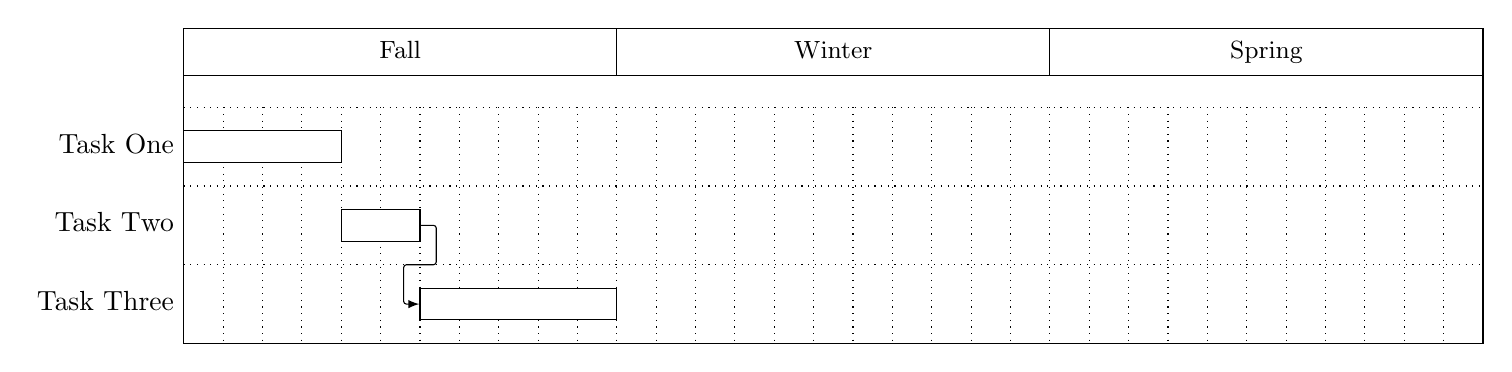
\begin{tikzpicture}[x=.5cm, y=2cm]
\begin{ganttchart}[vgrid, hgrid]{1}{33} % 3 terms
\gantttitle{Fall}{11} \gantttitle{Winter}{11} \gantttitle{Spring}{11} \\
\ganttbar{Task One}{1}{4} \\    
\ganttbar[name=b2]{Task Two}{5}{6} \\      
\ganttbar[name=b3]{Task Three}{7}{11}
\ganttlink{b2}{b3}
\end{ganttchart}
\end{tikzpicture}
}

\end{document}
